%%%%%%%%%%%%%%%%%%%%%%%%%%%%%%%%%%%%%%%%%%%%%%%%%%%%%%%%%%%%%%%%%%
%%%%%%%% ICML 2015 EXAMPLE LATEX SUBMISSION FILE %%%%%%%%%%%%%%%%%
%%%%%%%%%%%%%%%%%%%%%%%%%%%%%%%%%%%%%%%%%%%%%%%%%%%%%%%%%%%%%%%%%%

% Use the following line _only_ if you're still using LaTeX 2.09.
%\documentstyle[icml2015,epsf,natbib]{article}
% If you rely on Latex2e packages, like most modern people use this:
\documentclass{article}

% use Times
\usepackage{times}
% For figures
\usepackage{graphicx} % more modern
% \usepackage{epsfig} % less modern
\usepackage{subfigure} 

% For citations
\usepackage{natbib}

% For algorithms
\usepackage{algorithm}
\usepackage{algorithmic}

% As of 2011, we use the hyperref package to produce hyperlinks in the
% resulting PDF.  If this breaks your system, please commend out the
% following usepackage line and replace \usepackage{icml2015} with
% \usepackage[nohyperref]{icml2015} above.
\usepackage{hyperref}

% Packages hyperref and algorithmic misbehave sometimes.  We can fix
% this with the following command.
\newcommand{\theHalgorithm}{\arabic{algorithm}}

% Employ the following version of the ``usepackage'' statement for
% submitting the draft version of the paper for review.  This will set
% the note in the first column to ``Under review.  Do not distribute.''
% \usepackage{icml2015} 

% Employ this version of the ``usepackage'' statement after the paper has
% been accepted, when creating the final version.  This will set the
% note in the first column to ``Proceedings of the...''
\usepackage[accepted]{icml2015}

% Custom libraries.
\usepackage{amsmath}
\usepackage{amssymb}
\usepackage{bbm}
% Custom commands.
\DeclareMathOperator*{\argmin}{arg\,min}
\DeclareMathOperator*{\argmax}{arg\,max}
\newcommand{\R}{\mathbb{R}}
\newcommand{\X}{\mathbb{X}}
\newcommand{\x}{\mathbf{x}}
\newcommand{\y}{\mathbf{y}}
\newcommand{\D}{\mathcal{D}}
\newcommand{\N}[1]{\mathcal{N}\left(#1\right)}
\newcommand{\paren}[1]{\left({#1}\right)}
\newcommand{\brac}[1]{\left[{#1}\right]}
\renewcommand{\Pr}[1]{\mathbb{P}\brac{{#1}}}
\newcommand{\set}[1]{\left\{{#1}\right\}}
\newcommand{\T}{\boldsymbol{\Theta}}
\newcommand{\abs}[1]{\left|{#1}\right|}
\newcommand{\norm}[1]{\abs{\abs{{#1}}}_2^2}
\newcommand{\E}[1]{\mathbb{E}\left[#1\right]}

\newtheorem{theorem}{Theorem}[section]
\newtheorem{lemma}[theorem]{Lemma}
\newtheorem{proposition}[theorem]{Proposition}
\newtheorem{corollary}[theorem]{Corollary}
\newtheorem{claim}[theorem]{Claim}


% The \icmltitle you define below is probably too long as a header.
% Therefore, a short form for the running title is supplied here:
\title{Automated Statistician}
\icmltitlerunning{Automated Model Selection via Gaussian Processes}

\begin{document} 

\twocolumn[
\icmltitle{Automated Model Selection via Gaussian Processes}

% It is OKAY to include author information, even for blind
% submissions: the style file will automatically remove it for you
% unless you've provided the [accepted] option to the icml2015
% package.
\icmlauthor{Rui Shu}{rshu15@stanford.edu}
\icmlauthor{Stephen Koo}{sckoo@cs.stanford.edu}
\icmladdress{AA 228, Stanford University}

% You may provide any keywords that you 
% find helpful for describing your paper; these are used to populate 
% the "keywords" metadata in the PDF but will not be shown in the document
\icmlkeywords{bayesian optimization, acquisition functions}

\vskip 0.3in
]

\begin{abstract} 
In this paper, we tackle model selection by formulating the problem of hyperparameter optimization in the multi-model setting as a two-tiered system. The first tier is a multi-armed Gaussian Bandit problem that selects the model. The second tier is a Gaussian process-based Bayesian optimization technique that selects the optimal hyperparameters. We compare our model selection system to random search and demonstrated superior results. Our system extends on previous work in model selection, expanding model selection to include not only hyperparameter selection but also model family selection. We describe our system in detail and discuss future work for developing a more intelligent automated model selection system.
\end{abstract} 

\section{Introduction}
The desire to learn the a model in a fully automated way has been of considerable interest in the machine learning community \cite{deepfeature}. Much attention has been places on the automation of feature engineering; there has been a recent surge in the popularity of deep neural network architecture because of a DNN's ability to avoid feature engineering. However, these models often require large amounts of data to be trained properly, are computationally costly, are difficult to interpret and intuit, and require careful tuning of hyperparameters in order for the DNN to train successfully. 

Additionally, it is often a rule of thumb to start with a simple model before moving to more complex models on a case-by-case basis. But given the wide array of models that one can choose from, it is worth wondering whether it is possible to fully automate the predictive modeling process, providing automated selection of not only the optimal hyperparameters but also the optimal model for a given modeling task in the least amount of computational time.

\section{Hyperparameter Selection}
Many machine learning models requires the selection of hyperparameters \emph{a priori}. These hyperparameters are often critical to the performance of the model \cite{adams:prior} and reflect assumptions the model makes about the data distribution prior to training the model on the existing data. The most common approach to hyerparameter tuning involves cross-validation: using a given set of hyperparameters, a model is trained on training data and evaluated on a test set \cite{bengio}. The optimal set of hyperparameters is thus the hyerparameters that maximizes the model's performance on the test set. It is thus possible to consider the existence of a latent function $f$ that maps a given set of hyperparameters $\x \in \R^k$ to a performance metric. For a classification problem, this metric may, for example, be the accuracy of the model,
\begin{align}
  f(\x) = \frac{1}{N} \sum_{i=1}^N \mathbbm{1}\set{y_i = \hat{y}_i \mid \x},
\end{align}
where $y_i$ corresponds to the true label of the $i^{th}$ sample in the test set and $\hat{y}_i$ corresponds to label predicted by the trained model given hyerparameters $\x$. It is often the case that $f(\x)$ is observed with noise (resulting from any randomness associated with the training of the model), thus making it appropriate to reason about the expected value of $f$ instead.

\subsection{Gaussian Processes}
Since the goal to to find $\argmax_{\x} \E{f(\x)}$, the task of hyperparameter selection has often been formulated as a function optimization procedure performed using Gaussian process regression \cite{adams:practical}. Gaussian process regression is a non-parametric Bayesian modeling tool that imposes a prior distribution over $f$ and updates its belief about the distribution upon the observation of data. Formally, a Gaussian process is parameterized by a mean function $m(\x)$ and a kernel $k(\x, \x')$, which we define as,
\begin{align}
  m(\x) &= \E{f(\x)} \\
  k(\x, \x') &= \E{(f(\x) - m(\x))(f(\x') - m(\x'))},
\end{align}
which can be rewritten as $f(\x) \sim \mathcal{GP}(m(\x), k(\x, \x'))$. The exact choice of the functions $m$ and $k$ are priors required by the Gaussian process and the proper selection of such priors is describes in the next section. Crucially, a Gaussian process simply describes a collection of random variables $\set{f(\x_i)}_{1:n}$ drawn from a multivariate Gaussian distribution \cite{rasmussen:book}, and can thus be rewritten as,
\begin{align}
  \begin{bmatrix}
    f_1 \\ \vdots \\ f_n
  \end{bmatrix} \sim
  \N{\begin{bmatrix} m_1 \\ \vdots \\ m_n \end{bmatrix},
    \begin{bmatrix}
      k_{11} & \ldots & k_{1n} \\
      \vdots & \ddots & \vdots \\
      k_{n1} & \ldots & k_{nn}
  \end{bmatrix}},
\end{align}
where the dependency on $\x_{1:n}$ ($f_i = f(\x_i)$, $m_i = m(\x_i)$ and $k_{ij} = k(\x_i, \x_j)$) is suppressed for notational simplicity. For further simplicity, we write,
\begin{align}
  f_{1:n} \sim \N{m_{1:n}, k_{(1:n) \times (1:n)}}.
\end{align}

When seen as a multivariable Gaussian distributtion, it is easy to see how updating the Gaussian process involves computing a conditional Gaussian distribution. Supposing that the first $n-1$ points $f_{1:n-1}$ were observed, we compute the conditional distribution as,
\begin{align}
  \begin{bmatrix}
    f_{1:n-1} \\ f_n
  \end{bmatrix} &\sim
  \N{
    \begin{bmatrix} m_{1:n-1} \\  m_n \end{bmatrix},
    \begin{bmatrix}
      k_\alpha  & k_\beta \\
      k_\beta^\top  & k_\gamma
    \end{bmatrix}
  }, \\
  \begin{split}
    f_n \mid f_{1:n-1} &\sim
  \mathcal{N} (m_\D(x_n), k_\D(x_n, x_n)),
  \end{split}\\
  m_\D &= m_n + k_\beta^\top k_\alpha^{-1}(f_{1:n-1} - m_{1:n-1}), \\
  k_\D &= k_\gamma - k_\beta^\top k_\alpha^{-1} k_\beta,
\end{align}
where $k_\alpha = k_{(1:n-1) \times (1:n-1)}$, $k_\beta = k_{(1:n-1) \times n}$, and where $k_\gamma = k_{nn}$ \cite{rasmussen:lecture}. Here, $m_\D$ and $k_\D$ denote the posterior mean and covariance functions upon observation of the data $\D = f_{1:n-1}$. Since it is often the case that realizations of the random variables $f_{1:n-1}$ are observed with some $\sigma$-Gaussian noise, it is common to use $k_\alpha = k_{(1:n-1) \times (1:n-1)} + \sigma^2I_{n-1}$. Crucially, performing Gaussian process regression returns not only a posterior mean function, but also a posterior covariance function that properly captures the uncertainty of the interpolation. It is this ability of a Bayesian modeling tool to reason about the uncertainty of the system makes Gaussian processes for the online reinforcement learning task of function optimization \cite{sparse}.

\begin{figure*}
  \centering
  \subfigure[Gaussian process regression.]{\label{fig:sub1}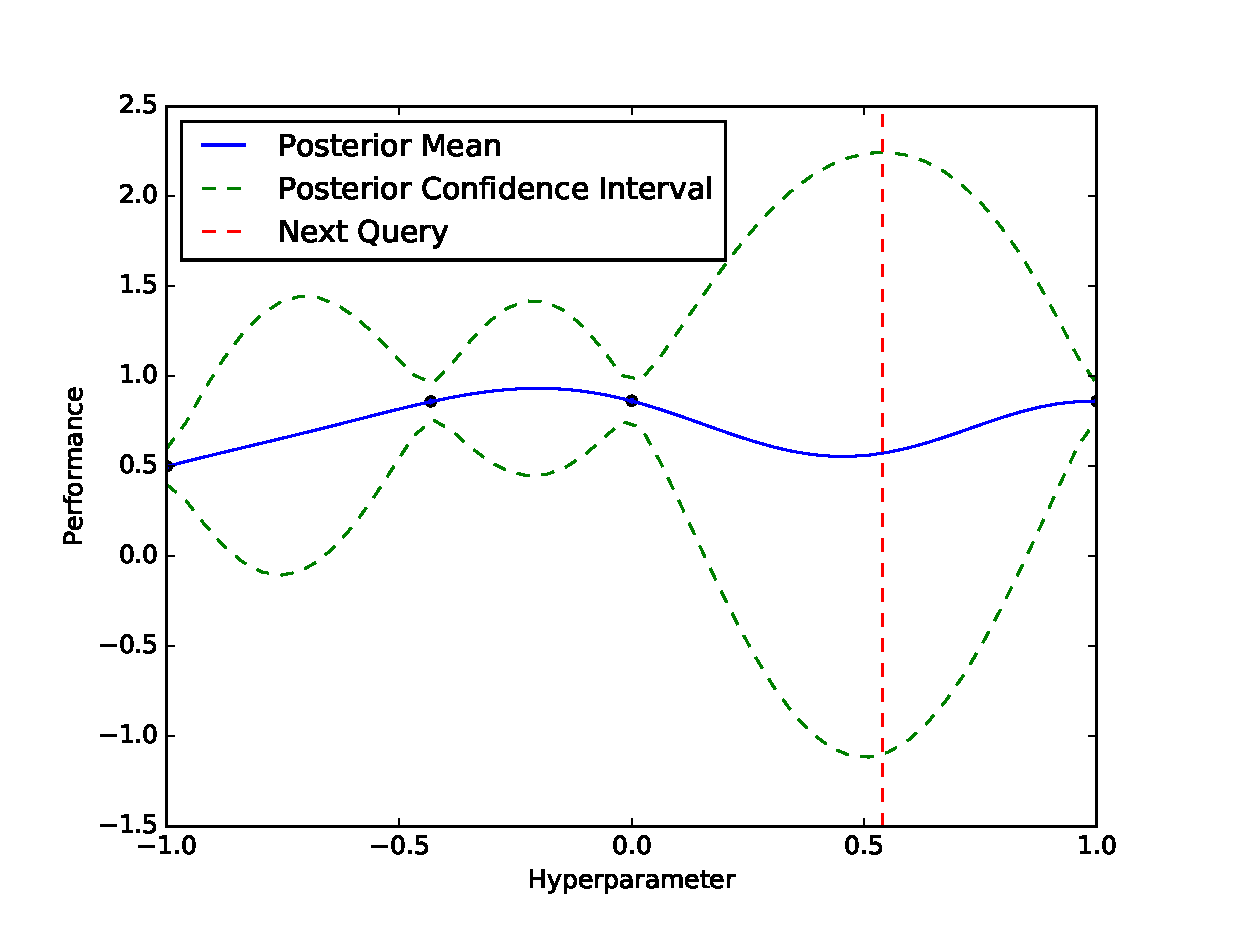
\includegraphics[width=.3\linewidth]{./images/bayesian_optimization.eps}}
  ~
  \subfigure[Model search comparison by iteration.]{\label{fig:sub2}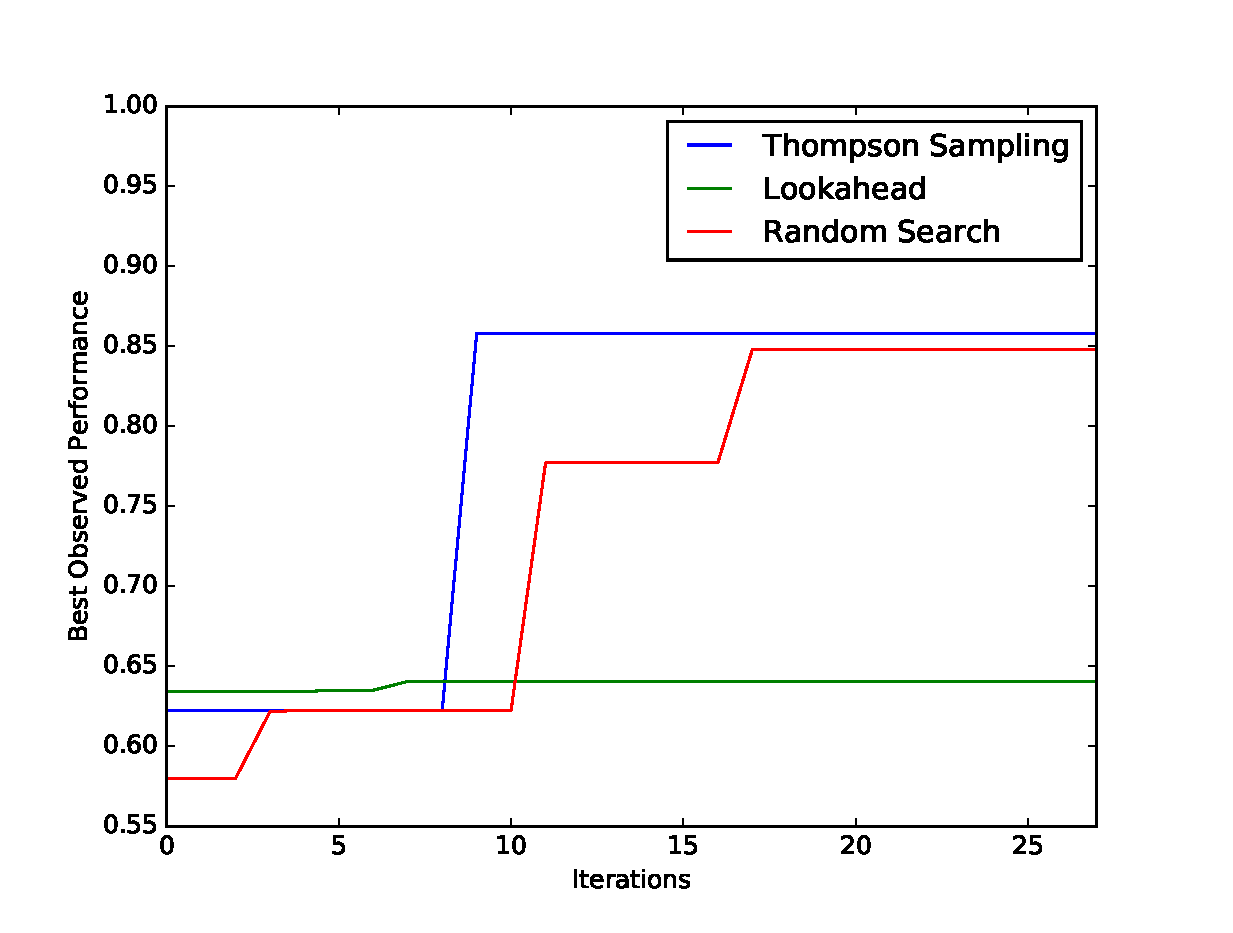
\includegraphics[width=.3\linewidth]{./images/iteration_based.eps}}
  ~
  \subfigure[Model search comparison by time elapsed.]{\label{fig:sub3}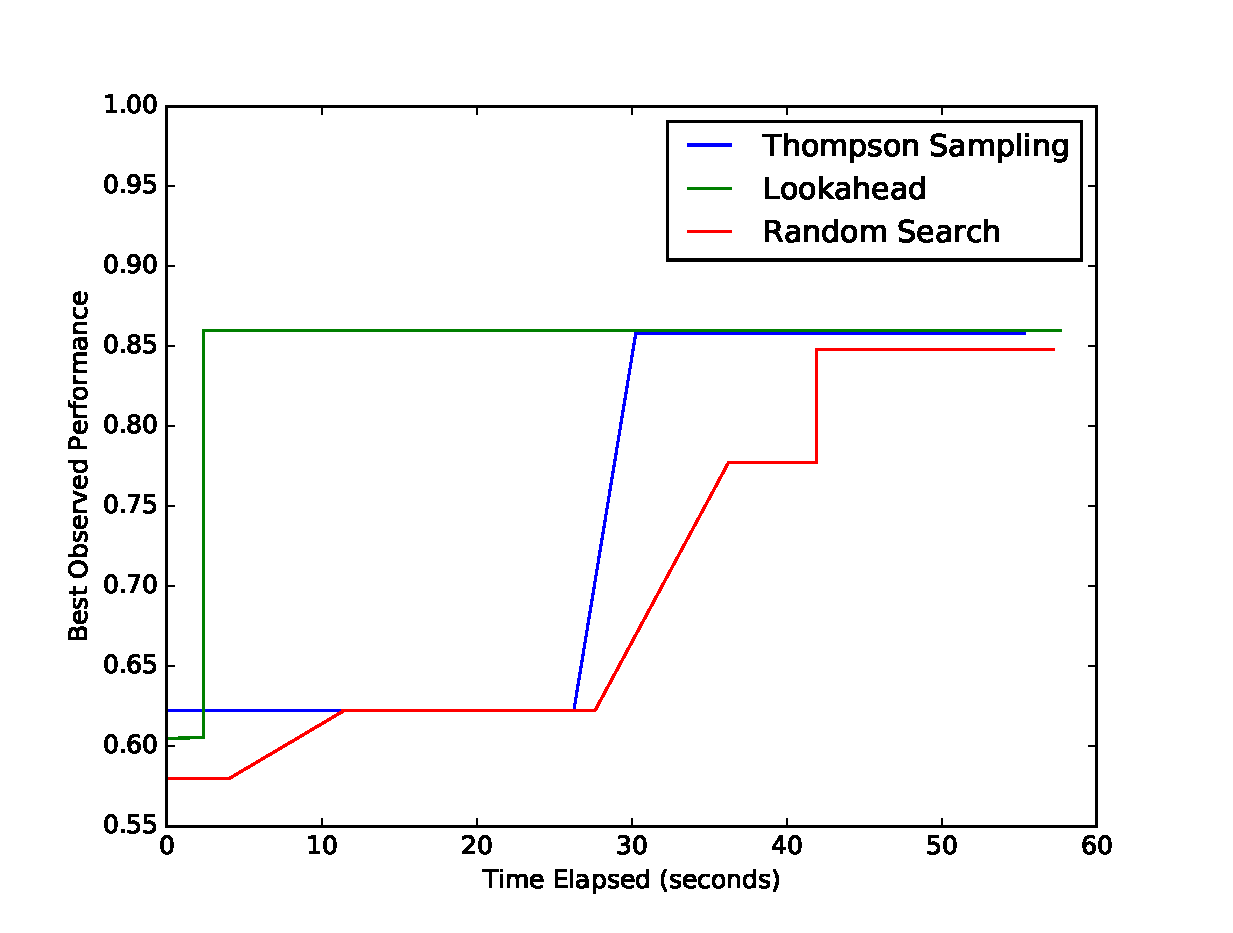
\includegraphics[width=.3\linewidth]{./images/time_based.eps}}

  \caption{In \ref{fig:sub1}, show an example Example Gaussian process fit of an unknown function, marked with the next point to query based on the computed maximum of the acquisition function. In \ref{fig:sub2} and \ref{fig:sub3}, we compare the model selection algorithms we present in this paper by plotting the trajectories of the best performance found with respect to the number of iterations (i.e. number of model-parameter combinations tried) and time elapsed. Note that \ref{fig:sub3} simply gives a different scaling of the same results, accounting for the differences between the training times required for different kinds of models.}
\end{figure*}

\subsubsection{Selection of Mean}
Despite being non-parameteric, a Gaussian process is not completely free-form and does require the imposition of certain priors, namely the mean and kernel functions. Since it is often the case that the regression task is performed within the unit hypercube, a zero-mean Gaussian process where $m(\x) = 0$ will often suffice and its impact on the posterior mean diminishes quickly with the introduction of more data. It is sometimes useful, however, to impose a quadractive prior if expert knowledge suggests that the optimal hyperparameters is unlikely to appear on the boundary constraints of the optimization task \cite{adams:prior}. 

\subsubsection{Selection of Kernel}
Perhaps of greater importance to the behavior of the Gaussian process is the kernel function. The choice of kernel functions can greatly impact the posterior mean and covariance of the Gaussian process. A plethora of kernel functions exist, ranging from periodic kernels to the Mat\'{e}rn and squared exponential kernel. Extensive research has been done on the performance of composite kernels generated from the linear combination of a set of basis kernels \cite{kernel}. Within the context of test-set performance function, however, if one is reasonably confident that the performance function varies smoothly over the hyperparameter space, it is often enough to impose the squared exponential kernel,
\begin{align}
  k(\x, \x') = \theta_0^2\exp\paren{-\frac{1}{2} \gamma\paren{\x, \x'}},
\end{align}
where $\gamma\paren{\x,\y}=\sum_{i=1}^k \frac{\paren{x_i-x'_i}^2}{\theta_i^2}$. It is still necessary to learn the parameters $\theta_{0:k}$. Of especial importance are the length scale parameters $\theta_{1:k}$, which reflect the extend to which observed points can influence the interpolation in its neighborhood. A large length scale reflects a greater sphere of influence, and vice versa. To learn these parameters, we choose the parameters $\theta_{0:k}$ that maximize the log marginal likelihood,
\begin{align}
  \begin{split}
    &\log p \left(f_{1:n} \vert \x_{1:n}, \theta_{0:k}\right) \propto \\
    &-(f_{1:n} - m_{1:n})^\top k_\alpha^{-1}(f_{1:n} - m_{1:n}) - \log \det k_\alpha,
  \end{split}
\end{align}
which can be performed via any gradient ascent algorithm \cite{rasmussen:lecture}. The term involving $\log \det k_\alpha$ can be interpreted as a regularization parameter that encourages longer length scales (i.e. a low variance model) as long as such simplicity does not greatly hinder the model's ability to fit the data, which is captured by the quadratic form $(f-m)^\top k_\alpha^{-1}(f-m)$. Since $k_\alpha$ is also a function of the noise parameter $\sigma$, it is also possible to learn the value of $\sigma$ via gradient ascent as well. However, introducing $\sigma$ as a learnable paramater often produces many local optima that reflects a different interpretation of the data; a large $\sigma$ is often accompanied by the learning of larger length scales, reflecting a low-variance high-bias interpolation, whereas a small $\sigma$ is accompanied by small length scales, reflecting a high-variance low-bias interpolation \cite{rasmussen:book}. Within the context of hyperparameter selection, the noise parameter is chosen beforehand and noted in the Experimental section.


\subsection{Sequential Hyperparameter Selection}
The use of a Gaussian process provides the Bayesian approach to modeling the uncertainty of the system, namely the confidence of our interpolated performance function. In an online function optimization framework, however, a sequential series of hyperparamters must be chosen, with the hope that each choice in the series allows us to make a more informed decision about the identity of the hyperparameters. To do so, it is important for the online system to properly manage exploration and exploitation. It is possible to formulate this task as a Belief-State Markov Decision Process (MDPs) where the belief-state is our belief about the latent performance function as capture by the Guassian process, the action-space is the set of all possible hyperparameters to choose from, and the observation-space is the set of all possible performance function evaluations at a particular hyperparameter. However, the continuous nature of the action and observation space makes most online methods intractable without discretization. It is thus common within the hyperparameter optimization literature to adopt the use of an acquisition function\textemdash a deterministic function of the posterior mean and covariance from the Gaussian process that allows for a simple albeit ad-hoc trade-off between exploration and exploitation \cite{adams:practical}. 

As is the case with kernel selection, many acquisition functions exist \cite{garnett}. In our experiments, we use the upper-confidence bound (UCB) for hyperparameter selection, defined as,
\begin{align}
  m_D(\x) + 2\sqrt{k_D(\x, \x)}.
\end{align}
The key benefit of such an acquisition function is that it is easily differentiable with respect to $\x$, enabling the use of gradient ascent to identify where the acquisition function is maximized without the need of evaluating the Gaussian process on a pre-defined grid of hyperparameters \cite{adams:practical}. 

\section{Model Selection}
While hyperparameter optimization has been extensively studied, there has been few research done on the hyperparameter optimization in a multi-model setting. Research in model selection has largely been focus on variable selection and hyperparameter tuning constrained within a single family of models, such as Random Forest \cite{deepfeature}. As the number of such approaches increases, it is natural to consider the possibility of extending the task of Bayesian optimization to include not only hyperparameter selection, but also model family selection. Here, we describe our formulation of the problem as an multi-armed Gaussian bandit. 

\subsection{Multi-Armed Gaussian Bandit}
A multi-armed Gaussian bandit problem addresses the question of optimal decision making where one sequentially selects from one of $N$ Gaussian distributions with unknown means and variances. In the bandit problem, the reward of each action is the observed realization from the chosen distribution. The multi-armed Gaussian bandit formulation of the model selection problem can be stated as follows.

Each sequential decision involves selecting both a model type (i.e. logistic regression, radius nearest-neighbors, etc.) and a set hyperparameters to initialize the model. The difficulty of performing model selection stems from the fact that each model type has an associated Gaussian process conditioned on the observations made thus far. However, note that we have predetermined our hyperparameter selection policy to be that of maximizing the UCB acquisition function. By doing so, we reduce our decision of which model down to that of selecting one of $N$ models at particular hyperparameter initializations. By looking at each model at a particular hyperparameter, we reduce the Gaussian process to a single Gaussian distribution for each model, thus avoiding the need to make a decision based on $N$ Gaussian processes.

\subsection{Sequential Model Selection}
As with sequential hyperparameter selection, there are many methods with which sequential model selection can be performed. The reduction of the problem to that of a multi-armed Gaussian bandit further opens up room for the use of various online methods available for Partially Observable Markov Decision Processes (POMDPs) \cite{mykel}. Of particular interest to us is to build a simple system that seeks a dynamic trade-off between exploration and exploitation dependent on the amount of time a user is willing to dedicate to automated model selection. Intuitively, the optimal policy ought to take into account a time limit imposed on the automated selection process; as the time limit gets smaller, the selection algorithm should become increasingly more conservative about querying computationally costly models. To reflect this, we define our reward function as follows,
\begin{align}
  R(a_t) =
  \begin{cases}
    o_t^{(f)} & o^{(t)}_t > 0 \\
    0 & o_t^{(t)} \le 0 
  \end{cases},
\end{align}
where $a_t$ is the model chosen at time $t$, yielding a 2-tuple observation $o_t = (o_t^{(f)}, o_t^{(t)})$ where $o_t^{(f)}$ is the observed performance of the model at the chosen hyperparameters $\x$, and $o_t^{(t)}$ is the amount of time left on the clock after the $t$ steps.

\subsubsection{Approximate Value Function Lookahead}
In the multi-armed Gaussian Bandit problem, the continuous obseravtion space still presents a challenge for optimal policy construction \cite{sparse}. One simple approach for tackling such a POMDP is to a one-step lookahead policy. Given a belief about the $N$ Gaussian distributions, we choose the action that maximizes the following expression,
\begin{align}
  R(b_t, a_t) + \gamma \frac{1}{n} \sum_{i=1}^n U(b_{t+1}^{(i)}),
\end{align}
where $b_{t+1}^{(i)}$ is the updated belief after simulating a virtual observation $o_t$ from the current belief-action pair. $U$ is the approximate value function which is approximated via a rollout evluation strategy described in \cite{mykel}. 

\subsubsection{Thompson Sampling}
Given current belief $b_t$ about the multi-armed Gaussian bandit, Thompson sampling samples a observation of each of the $N$ Gaussian distribution based on our current belief and simply performs the action that maximizes the reward. This simple approach is effective despite its simplicity and has often outperforms competing techniques. However, it is known that Thompson sampling is still a myopic selection strategy and is prone to overexploration \cite{sparse}.

\begin{figure}
  \vspace{0pt}
  \centering
  \subfigure[Thompson Sampling model selection.]{\label{fig:sub4}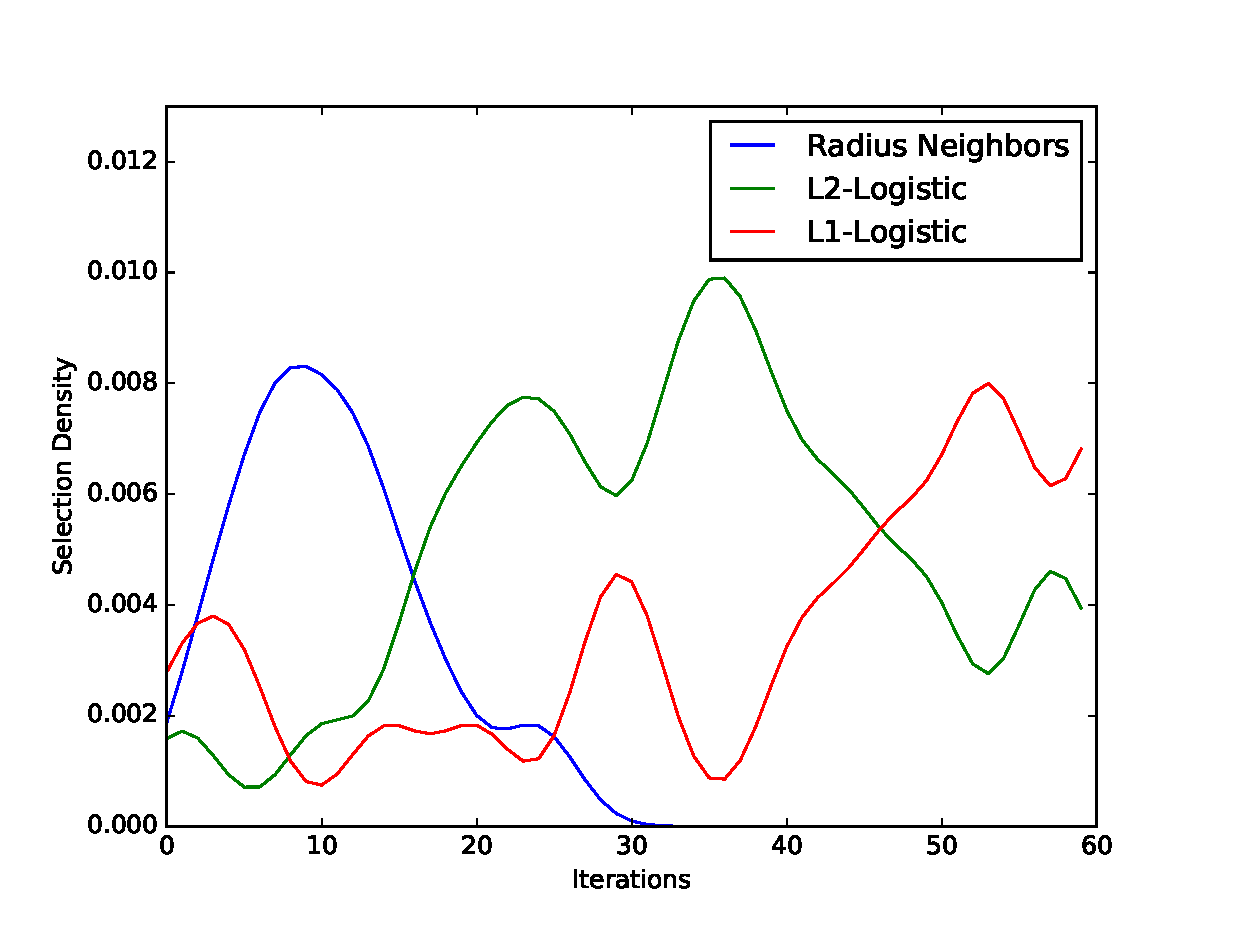
\includegraphics[width=.7\linewidth]{./images/density_thompson_sampling.eps}}
  ~
  \subfigure[Lookahead model selection.]{\label{fig:sub5}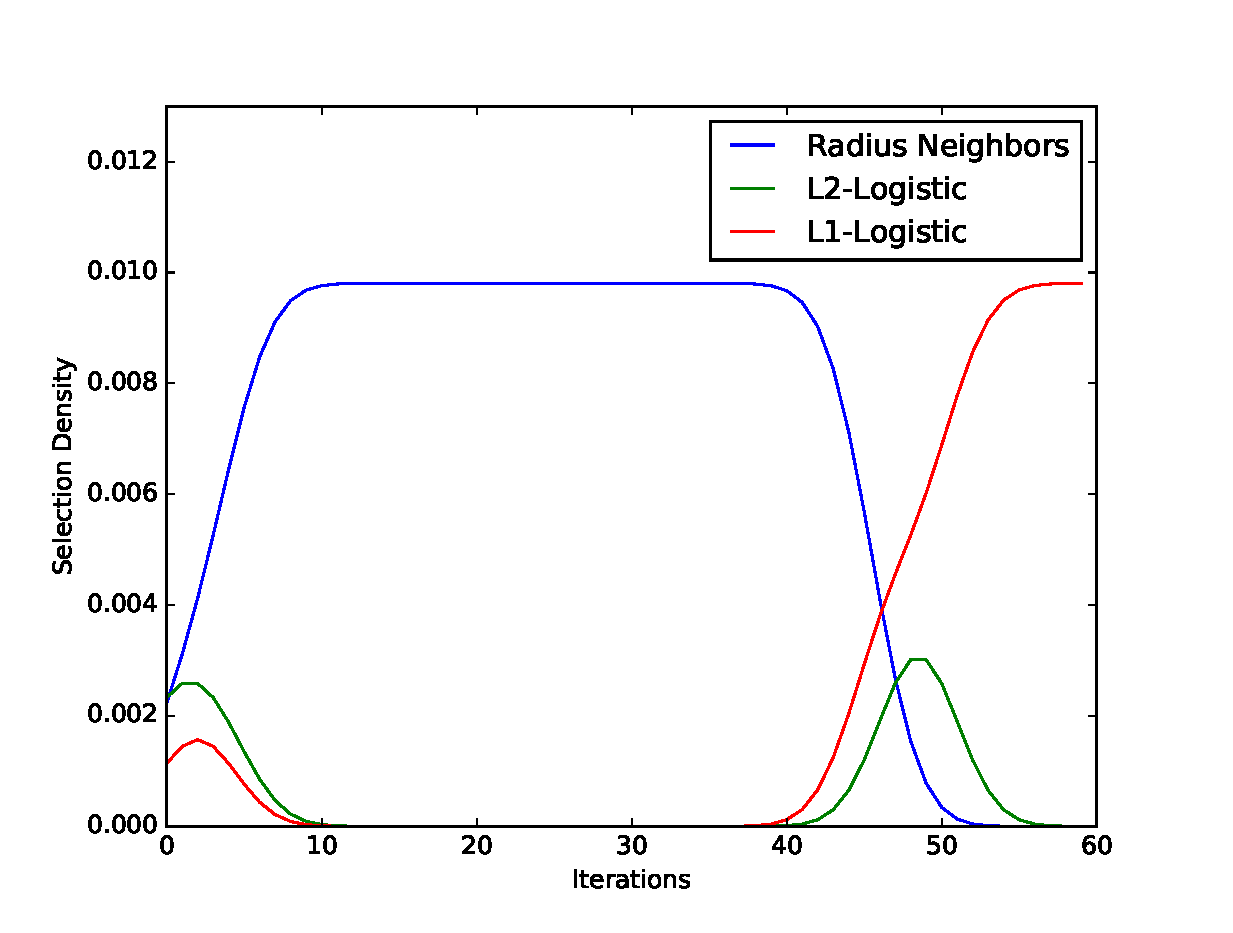
\includegraphics[width=.7\linewidth]{./images/density_lookahead.eps}}
  
  \caption{In these figures we chart the frequency with which each model is tried by the respective algorithms. For visualization purposes, we use Gaussian kernel density estimation to estimate the density of these selection events with respect to the cumulative number of tries.}
\end{figure}

\section{Experiments}
\subsection{Experimental Details}
\label{exp}
To evaluate the performance of our online multi-model selection algorithm, we evaluated three models, L1-logistic regression L2-logistic regression, and Radius Neighbors classifier on a synthetic binary classification dataset containing $10000$ samples. The samples were generated from a mixture of four Gaussian distributions and labeled according to the XOR labeling scheme. As such, the data set is not linearly separable. Each model contained a single hyperparameter, namely the penalty hyperparameter for the logistic regressions and the radius for the Radius Neighbors classifier.

We ran three different three different model selection algorithms. We used pure random search as our baseline. Despite its simplicity, random search is often used for hyperparameter selection and serves as a minimal baseline for our multi-model selection task \cite{bengio}. The random search algorithm randomly selects a model and a single set of hyperparameter at each iteration. We then used two flavors of our proposed multi-model selection algorithm. The first implements sequential model selection using lookahead with approximate value function, while the second uses Thompson sampling. Both versions iteratively selects a single model type (according to their respective methods) as well as a single hyperparameter using the UCB acquisition function.

All three selection strategies were tested with a fixed time limit of $60$ seconds for model training and testing. The imposition of the time limit for this example problem simulates the situation in reality when model selection and hyperparameter selection are costly operations that make take many hours to run. Under these circumstances, the balance of exploitation and exploration ought to change depending on the amount of time allowed for the optimization task as well as the differential computation cost of each family of models.

\subsection{Results}
Our results demonstrate that both model selection approaches (Thompson sampling and Approximate Value Function Lookahead) are superior to random search. As can be see in Figures \ref{fig:sub2} and \ref{fig:sub3}, our selection techniques found the optimal model and hyperparameters in a significantly smaller number of queries than random search, thus reducing the number of expensive model performance computation queries. The ability of our selection system to quickly identify the optimal hyperparameter in a multi-model setting will be of significantly greater value when scaled to tackle truly complex models with costly cross-validation performance evaluations. 

It is also interesting to compare the differences in the behavior of the model selection system when using Thompson sampling as compared to Approximate Value Function Lookahead. Both consistently exploit the best-performing model at the beginning. Since the data set is not linearly separable, the non-parametric Radius Neighbors classifier significantly outperforms logistic regression when its hyperparameter is carefully chosen. However, because Radius Neighbors classifier is computationally more costly than logistic regression (the Radius Neighbors has a run-time complexity of $O(n^2)$ while logistic regression has a run-time complexity of $O(p)$ where $n$ is the number of samples and $p$ is the number of predictors in the dataset), both model selection systems favor the simpler models as we approach the time limit. However, the two systems exhibit very different behaviors in the middle. Figures \ref{fig:sub4} and \ref{fig:sub5} show that Thompson Sampling is more likely to explore all three model types than Approximate Value Function Lookahead. This difference in behavior is consistent with Thompson sampling's known tendency to over-explore.

\section{Discussion}
We demonstrated two simple but successful ways of extending automated machine learning to that of the multi-model level by leveraging Bayesian-theoretic approaches toward reinforcement learning. The two-tier approach we propose for model and hyperparameter selection is highly flexible and can be readily modified to meet the needs of the user. Here, we propose future work that will improve upon our proposed system.

\subsection{Bayesian Selection Techniques}
We demonstrated the use of the UCB acquisition function, Thompson sampling, and Approximate Value Function Lookahead for the purposes of online hyperparameter and model selection. We directly compared Thompson sampling with Approximate Value Function Lookahead and demonstrated Thompson sampling's tendency to overexplore. While Approximate Value Function Lookahead reduces the risk of overexploration, it is nevertheless a crude technique for approximating the optimal value function associated with a given belief state. Other techniques, such as sparse sampling and Monte Carlo Tree Search has been proposed to deal with POMDPs with continuous observation space \cite{adaptive}. It is conceivable that some of these more popular techniques for handling POMDPs will yield policies that better approximate the true optimal policy.

\subsection{Reward Function Determination}
Thus far, we implemented a fairly simplistic reward function. One of our goals for an automated model selection system, however, is for the system to adapt to the user's time and resource constraints, as well as any additional preferences the user may have of model complexity. For instance, if the user wishes to severely penalize the selection of a complex model, the reward function should be adjusted accordingly. One possibility is additively include a penalty term such as the Bayesian Information Criterion (BIC). The exact formulation of the reward function for automated model selection is worthy of exploration and an analysis of the model selection behavior under different types of reward function will allow us to tailor a reward function according to a user's needs.

\subsection{Inter-Model Covariance}
Our existing system uses a single Gaussian process for each model type. As it stands, observations from one model does not influence the Gaussian processes associated with other models. However, it is easy to intuit that the performance of one model on a given dataset can sometimes inform us about the expected performance of a closely-related model. For example, the performance of L1-logistic regression should inform us about the performance of L2-logistic regression. In other words, it is not surprising for the performances of two models to have non-zero covariances across datasets. Since a Gaussian process is formally simply a collection of random variables and is agnostic toward the the random variables coming from different sources \cite{rasmussen:book}, it is not out of the question to incorporate out-of-family model performances into the Gaussian process. The main challenge of incoporating inter-model information stems from the choice of the covariance terms. Since the external model information comes from separate hyperparameter space, it is not possible to use a distance-based kernel function to approximate the inter-model covariance terms. However, these covariances can be learned via maximum likelihood estimation by training all models on a variety of datasets. With these additional research avenues, it is possible for our automated selection system to perform even better.
\bibliography{main}
\bibliographystyle{icml2015}
\end{document} 


